% Options for packages loaded elsewhere
\PassOptionsToPackage{unicode}{hyperref}
\PassOptionsToPackage{hyphens}{url}
%
\documentclass[
  12pt,
  a4paper,
  oneside]{book}
\usepackage{amsmath,amssymb}
\usepackage[]{lmodern}
\usepackage{iftex}
\ifPDFTeX
  \usepackage[T1]{fontenc}
  \usepackage[utf8]{inputenc}
  \usepackage{textcomp} % provide euro and other symbols
\else % if luatex or xetex
  \usepackage{unicode-math}
  \defaultfontfeatures{Scale=MatchLowercase}
  \defaultfontfeatures[\rmfamily]{Ligatures=TeX,Scale=1}
  \setmonofont[]{Menlo}
\fi
% Use upquote if available, for straight quotes in verbatim environments
\IfFileExists{upquote.sty}{\usepackage{upquote}}{}
\IfFileExists{microtype.sty}{% use microtype if available
  \usepackage[]{microtype}
  \UseMicrotypeSet[protrusion]{basicmath} % disable protrusion for tt fonts
}{}
\makeatletter
\@ifundefined{KOMAClassName}{% if non-KOMA class
  \IfFileExists{parskip.sty}{%
    \usepackage{parskip}
  }{% else
    \setlength{\parindent}{0pt}
    \setlength{\parskip}{6pt plus 2pt minus 1pt}}
}{% if KOMA class
  \KOMAoptions{parskip=half}}
\makeatother
\usepackage{xcolor}
\IfFileExists{xurl.sty}{\usepackage{xurl}}{} % add URL line breaks if available
\IfFileExists{bookmark.sty}{\usepackage{bookmark}}{\usepackage{hyperref}}
\hypersetup{
  pdftitle={Meine Master Arbeit},
  pdfauthor={Aweseome Boii},
  hidelinks,
  pdfcreator={LaTeX via pandoc}}
\urlstyle{same} % disable monospaced font for URLs
\usepackage[left=25mm,right=20mm,top=25mm,bottom=25mm]{geometry}
\usepackage{color}
\usepackage{fancyvrb}
\newcommand{\VerbBar}{|}
\newcommand{\VERB}{\Verb[commandchars=\\\{\}]}
\DefineVerbatimEnvironment{Highlighting}{Verbatim}{commandchars=\\\{\}}
% Add ',fontsize=\small' for more characters per line
\usepackage{framed}
\definecolor{shadecolor}{RGB}{248,248,248}
\newenvironment{Shaded}{\begin{snugshade}}{\end{snugshade}}
\newcommand{\AlertTok}[1]{\textcolor[rgb]{0.94,0.16,0.16}{#1}}
\newcommand{\AnnotationTok}[1]{\textcolor[rgb]{0.56,0.35,0.01}{\textbf{\textit{#1}}}}
\newcommand{\AttributeTok}[1]{\textcolor[rgb]{0.77,0.63,0.00}{#1}}
\newcommand{\BaseNTok}[1]{\textcolor[rgb]{0.00,0.00,0.81}{#1}}
\newcommand{\BuiltInTok}[1]{#1}
\newcommand{\CharTok}[1]{\textcolor[rgb]{0.31,0.60,0.02}{#1}}
\newcommand{\CommentTok}[1]{\textcolor[rgb]{0.56,0.35,0.01}{\textit{#1}}}
\newcommand{\CommentVarTok}[1]{\textcolor[rgb]{0.56,0.35,0.01}{\textbf{\textit{#1}}}}
\newcommand{\ConstantTok}[1]{\textcolor[rgb]{0.00,0.00,0.00}{#1}}
\newcommand{\ControlFlowTok}[1]{\textcolor[rgb]{0.13,0.29,0.53}{\textbf{#1}}}
\newcommand{\DataTypeTok}[1]{\textcolor[rgb]{0.13,0.29,0.53}{#1}}
\newcommand{\DecValTok}[1]{\textcolor[rgb]{0.00,0.00,0.81}{#1}}
\newcommand{\DocumentationTok}[1]{\textcolor[rgb]{0.56,0.35,0.01}{\textbf{\textit{#1}}}}
\newcommand{\ErrorTok}[1]{\textcolor[rgb]{0.64,0.00,0.00}{\textbf{#1}}}
\newcommand{\ExtensionTok}[1]{#1}
\newcommand{\FloatTok}[1]{\textcolor[rgb]{0.00,0.00,0.81}{#1}}
\newcommand{\FunctionTok}[1]{\textcolor[rgb]{0.00,0.00,0.00}{#1}}
\newcommand{\ImportTok}[1]{#1}
\newcommand{\InformationTok}[1]{\textcolor[rgb]{0.56,0.35,0.01}{\textbf{\textit{#1}}}}
\newcommand{\KeywordTok}[1]{\textcolor[rgb]{0.13,0.29,0.53}{\textbf{#1}}}
\newcommand{\NormalTok}[1]{#1}
\newcommand{\OperatorTok}[1]{\textcolor[rgb]{0.81,0.36,0.00}{\textbf{#1}}}
\newcommand{\OtherTok}[1]{\textcolor[rgb]{0.56,0.35,0.01}{#1}}
\newcommand{\PreprocessorTok}[1]{\textcolor[rgb]{0.56,0.35,0.01}{\textit{#1}}}
\newcommand{\RegionMarkerTok}[1]{#1}
\newcommand{\SpecialCharTok}[1]{\textcolor[rgb]{0.00,0.00,0.00}{#1}}
\newcommand{\SpecialStringTok}[1]{\textcolor[rgb]{0.31,0.60,0.02}{#1}}
\newcommand{\StringTok}[1]{\textcolor[rgb]{0.31,0.60,0.02}{#1}}
\newcommand{\VariableTok}[1]{\textcolor[rgb]{0.00,0.00,0.00}{#1}}
\newcommand{\VerbatimStringTok}[1]{\textcolor[rgb]{0.31,0.60,0.02}{#1}}
\newcommand{\WarningTok}[1]{\textcolor[rgb]{0.56,0.35,0.01}{\textbf{\textit{#1}}}}
\usepackage{graphicx}
\makeatletter
\def\maxwidth{\ifdim\Gin@nat@width>\linewidth\linewidth\else\Gin@nat@width\fi}
\def\maxheight{\ifdim\Gin@nat@height>\textheight\textheight\else\Gin@nat@height\fi}
\makeatother
% Scale images if necessary, so that they will not overflow the page
% margins by default, and it is still possible to overwrite the defaults
% using explicit options in \includegraphics[width, height, ...]{}
\setkeys{Gin}{width=\maxwidth,height=\maxheight,keepaspectratio}
% Set default figure placement to htbp
\makeatletter
\def\fps@figure{htbp}
\makeatother
\setlength{\emergencystretch}{3em} % prevent overfull lines
\providecommand{\tightlist}{%
  \setlength{\itemsep}{0pt}\setlength{\parskip}{0pt}}
\setcounter{secnumdepth}{5}
% Überschriften, Inhaltsverzeichnisse, etc. auf Deutsch
\usepackage[ngerman]{babel}

% Text unter Abbildungen, Tabellen, etc.
\usepackage[indention=1cm,format=plain,textformat=simple,labelformat=simple,labelfont=footnotesize,textfont=footnotesize,position=bottom]{caption}
\captionsetup[table]{position=below}

% Schönere Tabellen
\usepackage{booktabs}

% Bessere Mathe-Funktionalitäten
% Fixt ein paar Mathe-Renderprobleme bei amsmath
\usepackage{mathtools}

% Hier um Spalten einer Tabelle fett zu machen
\usepackage{array}
\usepackage{tabu}

% Titel, Author, Datum kann mit \thetitle, \theauthor, \thedate aufgerufen werden
\usepackage{titling}

% Kopf- und Fußzeile
\usepackage{fancyhdr}
% Kopf- und Fußzeile für Abstrakt, Deklaration und Inhaltsverzeichnis
\pagestyle{fancy}
\fancyhf{} % alles bereinigen
\fancyhead[L]{\nouppercase{\leftmark}} % Kopfzeile links
\fancyhead[C]{} %zentrierte Kopfzeile
\fancyhead[R]{\thepage} %Kopfzeile rechts
\setlength{\headheight}{15pt}
\renewcommand{\headrulewidth}{0.4pt} %obere Trennlinie

\fancypagestyle{plain}{%
  \fancyhf{} %alle Kopf- und Fußzeilenfelder bereinigen
  \fancyhead[R]{\thepage} %Kopfzeile rechts
}


% Layout bzw. Text für Kapitelüberschriften
\usepackage{titlesec}
\titleformat{\chapter}[hang]{\normalfont\huge\bfseries}{\thechapter\ }{1em}{}

% Listing Captions
\usepackage{floatrow}
\DeclareNewFloatType{listing}{placement=H, fileext=lsts, name=}
\captionsetup{options=listing}
\renewcommand{\thelisting}{\thechapter.\arabic{listing}}
\makeatletter
\@addtoreset{listing}{chapter}
\makeatother
\newcommand{\codeblock}[2]{\refstepcounter{listing}\label{#1}Listing~\thelisting: #2\vspace{-10pt}}
\newcommand{\lstbeg}[2]{\begingroup\begin{center}\codeblock{#1}{#2}\phantomsection\addcontentsline{lsts}{figure}{Listing \thelisting: #2}\end{center}}
\newcommand{\lstend}{\endgroup}

% Inhaltsverzeichnis für Listings
\makeatletter
%\newcommand\listingname{Listings}
\newcommand\listoflistings{%
  \chapter*{Listings}\@starttoc{lsts}}
\makeatother

% 1,5-facher Zeilenabstand
\usepackage[onehalfspacing]{setspace}
% Zeileneinzug nach jedem Paragraphen
\setlength{\parindent}{15pt}
% Zusätzlicher Zeilenabstand nach jedem Paragraphen
\setlength{\parskip}{0pt}

% Zitierformat
\usepackage{natbib}
\setcitestyle{numbers}
\setcitestyle{square}

% maketitle soll nicht angezeigt werden, Titelseite wird mit frontpage.tex generiert
\AtBeginDocument{\let\maketitle\relax}
\ifLuaTeX
  \usepackage{selnolig}  % disable illegal ligatures
\fi
\usepackage[]{natbib}
\bibliographystyle{plainnat}

\title{Meine Master Arbeit}
\author{Aweseome Boii}
\date{30.09.2022}

\begin{document}
\frontmatter
\maketitle

\thispagestyle{empty}

% Graphics
\begin{figure}[t]
 \raggedleft
 
\includegraphics[width=0.4\textwidth]{imgs/logo.jpg}
\end{figure}


% \begin{verbatim}
% \end{verbatim}

% \begin{center}
% \Large{Fachhochschule Kempten}\\
% \Large{- Campus <Name> -}\\
% \end{center}


% \begin{center}
% \Large{Faculty of Computer Science}
% \end{center}
% \begin{verbatim}
% \end{verbatim}
% Document title

\onehalfspacing
\begin{center}
    \textbf{\large{Master's Thesis}}\\
    \large{Computer Science}\\
    \vspace{50pt}

    \textbf{\LARGE{\thetitle}}\\
    \vspace{50pt}

    \large{\theauthor}\\
    \vspace{150pt}
\end{center}

\begin{flushleft}
    \begin{tabular}{>{\bfseries}ll}
        Institution & Augsburg Uni \\
        Degree & Master of Science (M.Sc.) \\
        Author Name & \theauthor \\
        Matr. Nr. & 325693 \\
        Address & Stützeweg 7 \\
        & 6993 Mittelberg \\
        & Austria \\
        Contact & felix.w.fritz@stud.hs-kempten.de \\
        & 0176 2412 1368 \\
        & \\
        1. Examiner & Prof.\ Dr.\ Jochen Staudacher \\
        2. Examiner & Prof.\ Dr.\ Jürgen Brauer \\
        Submission Date & \thedate
    \end{tabular}
\end{flushleft}

\mainmatter
\newpage

\frontmatter

\hypertarget{deklaration}{%
\chapter*{Deklaration}\label{deklaration}}

I hereby declare and confirm that this thesis is entirely the result of
my own original work. Where other sources of information have been used,
they have been indicated as such and properly acknowledged. I further
declare that this or similar work has not been submitted for credit
elsewhere.

\vspace{30pt}

\begin{tabu} to \linewidth {>{}X>{\centering}X}
 & \\
Augsburg, \thedate & \makebox[1\linewidth]{\dotfill}\\
 & {\small \textit{\theauthor}}\\
\end{tabu}

\hypertarget{kurzzusammenfassung}{%
\chapter*{Kurzzusammenfassung}\label{kurzzusammenfassung}}

In many situations, ranking agents or items based on their performance
within groups is of big interest. While it is possible to utilize power
indexes from cooperative game theory to solve such tasks, they require
every coalition to have a numerical value attached to them. Trying to
factor in all information that contributes to these values can be an
impossible task in real-life complex systems. Social rankings build a
framework that provides remedy to these complex structures by solely
relying on the ordinal ranking of coalitions, through which a power
relation between elements can be established.

Because the concept of social ranking solutions has been introduced only
recently, no general-purpose software exists to calculate these yet.
With the goal of developing an R package to solve these problems, this
thesis looks to build a foundational understanding of relations, orders,
and solutions, before delving into the package implementation itself.

\tableofcontents
\listoffigures
\listoftables
\listoflistings

\mainmatter

\hypertarget{einfuxfchrung}{%
\chapter{Einführung}\label{einfuxfchrung}}

\hypertarget{motivation}{%
\section{Motivation}\label{motivation}}

Darum machen wir das.

\hypertarget{vorgeschichte}{%
\section{Vorgeschichte}\label{vorgeschichte}}

Wie alles begann.

\hypertarget{etwas}{%
\chapter{Etwas}\label{etwas}}

Ich zitiere Moretti \citep{2017Moretti}, Khani \citep{2019Khani} oder
beide \citep{2017Moretti, 2019Khani}.

\newpage

\hypertarget{neue-seite}{%
\section{Neue Seite}\label{neue-seite}}

Dort wurde ein Seitenumbruch eingefügt.

\hypertarget{mehr}{%
\chapter{Mehr}\label{mehr}}

Noch mehr Formel in (\ref{eq:abc}).\footnote{Diese Formel ist nicht
  ernst zu nehmen.}

\begin{equation}\label{eq:abc}
a^2 + b^2 = c^2
\end{equation}

\hypertarget{implementierung}{%
\chapter{Implementierung}\label{implementierung}}

Hier sehen wir uns die Implementierung an, siehe Abb. \ref{fig:badges}
für die Darstellung auf GitHub..

\begin{figure}
\hypertarget{fig:badges}{%
\centering
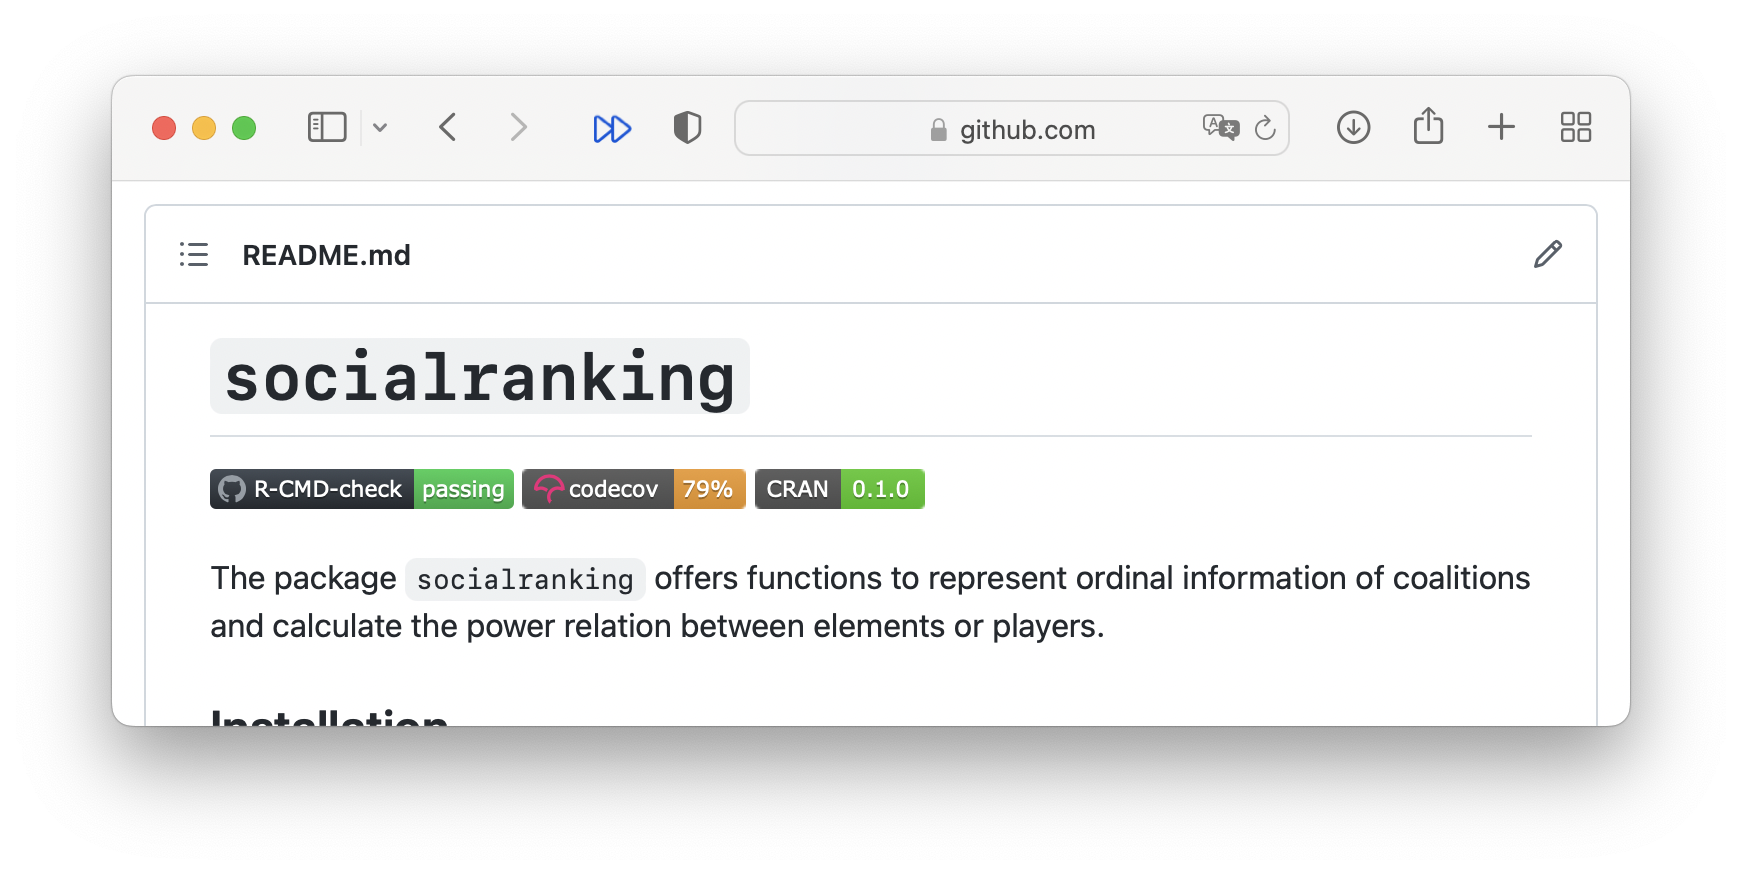
\includegraphics[width=0.6\textwidth,height=\textheight]{imgs/github_badges.png}
\caption{GitHub Badges}\label{fig:badges}
}
\end{figure}

\hypertarget{diskussion}{%
\chapter{Diskussion}\label{diskussion}}

War das nun eine gute Idee? Wir werden es wohl nie erfahren\(\cdots\).

\hypertarget{fazit}{%
\chapter{Fazit}\label{fazit}}

Hier bin ich auf folgendes Fazit gestoßen.

\backmatter

\newpage
\phantomsection\addcontentsline{toc}{chapter}{Bibliography}
\bibliography{refs.bib}

\setcounter{chapter}{1}
\renewcommand{\thechapter}{\Alph{chapter}}
\renewcommand{\thesection}{A.\arabic{section}}
\renewcommand{\thesubsection}{A.\arabic{section}.\arabic{subsection}}

\hypertarget{appendix}{%
\chapter{Appendix}\label{appendix}}

\hypertarget{plus-aufgaben}{%
\section{Plus-Aufgaben}\label{plus-aufgaben}}

Probier dies.

\lstbeg{code:plus}{Plusaufgaben lösen}

\begin{Shaded}
\begin{Highlighting}[numbers=left,,]
\NormalTok{pl }\OtherTok{\textless{}{-}} \DecValTok{5}
\NormalTok{pl }\SpecialCharTok{+} \DecValTok{3}
\DocumentationTok{\#\# [1] 8}
\end{Highlighting}
\end{Shaded}

\lstend

\hypertarget{minus-aufgaben}{%
\section{Minus-Aufgaben}\label{minus-aufgaben}}

Das war wirklich schwer zu lösen.

\lstbeg{code:minus}{Minusaufgaben lösen}

\begin{Shaded}
\begin{Highlighting}[numbers=left,,]
\NormalTok{ll }\OtherTok{\textless{}{-}} \DecValTok{5}
\NormalTok{ll }\SpecialCharTok{{-}} \DecValTok{3}
\DocumentationTok{\#\# [1] 2}
\end{Highlighting}
\end{Shaded}

\lstend

\newpage

\hypertarget{mit-python}{%
\section{Mit Python}\label{mit-python}}

\lstbeg{code:python}{Eine Python Aufgabe}

\begin{Shaded}
\begin{Highlighting}[numbers=left,,]
\NormalTok{arr }\OperatorTok{=}\NormalTok{ [}\StringTok{\textquotesingle{}hey\textquotesingle{}}\NormalTok{, }\StringTok{\textquotesingle{}mum\textquotesingle{}}\NormalTok{]}
\CommentTok{\textquotesingle{}, \textquotesingle{}}\NormalTok{.join(arr)}
\CommentTok{\#\# \textquotesingle{}hey, mum\textquotesingle{}}
\end{Highlighting}
\end{Shaded}

\lstend

\backmatter
\end{document}
